\documentclass[a4paper,oneside,14pt]{extarticle}

\usepackage{cmap} % Улучшенный поиск русских слов в полученном pdf-файле
\usepackage[T2A]{fontenc} % Поддержка русских букв
\usepackage[utf8]{inputenc} % Кодировка utf8
\usepackage[english,russian]{babel} % Языки: русский, английский

\usepackage[14pt]{extsizes}

\usepackage{graphicx}
\usepackage{multirow}

\usepackage{tikz}
\usetikzlibrary{shapes, shapes.geometric, arrows, arrows.meta, positioning}

\usepackage{caption}
\captionsetup{labelsep=endash}
\captionsetup[figure]{name={Рисунок}}

\usepackage{amsmath}
\usepackage{amsfonts}

\usepackage{geometry}
\geometry{left=30mm}
\geometry{right=10mm}
\geometry{top=20mm}
\geometry{bottom=20mm}

\usepackage{enumitem}

\usepackage{tabularx}
\usepackage{longtable}
\usepackage{adjustbox}
\usepackage{threeparttable}

% Переопределение стандартных \section, \subsection, \subsubsection по ГОСТу;
\usepackage{titlesec}[explicit]
\titleformat{name=\section,numberless}[block]{\normalfont\large\bfseries\centering}{}{0pt}{}
\titleformat{\section}[block]{\normalfont\large\bfseries}{\thesection}{1em}{}
\titlespacing\section{\parindent}{*4}{*4}

\titleformat{\subsection}[hang]
{\bfseries\large}{\thesubsection}{1em}{}
\titlespacing\subsection{\parindent}{*2}{*2}

\titleformat{\subsubsection}[hang]
{\bfseries\large}{\thesubsubsection}{1em}{}
\titlespacing\subsubsection{\parindent}{*2}{*2}

\usepackage{url}

% Переопределение их отступов до и после для 1.5 интервала во всем документе
\usepackage{setspace}
\onehalfspacing % Полуторный интервал
\frenchspacing
\setlength\parindent{1.25cm}

\usepackage{indentfirst} % Красная строка

% Настройки оглавления
\usepackage{xcolor}
\usepackage{multirow}

% Гиперссылки
\usepackage[pdftex]{hyperref}
\hypersetup{hidelinks}

% Дополнительное окружения для подписей
\usepackage{array}
\newenvironment{signstabular}[1][1]{
	\renewcommand*{\arraystretch}{#1}
	\tabular
}{
	\endtabular
}

\usepackage{enumitem} 
\setenumerate[0]{label=\arabic*)} % Изменение вида нумерации списков
\renewcommand{\labelitemi}{---}

% Листинги 
\usepackage{courier}
\usepackage{listings}
\usepackage{chngcntr} % Listings counter within section set main.tex after begin document
\usepackage{float} % Place figures anywhere you want; ignore floating
\floatstyle{plaintop}
\newfloat{code}{H}{myc}

% Для листинга кода:
\lstset{
	basicstyle=\small\ttfamily,			% размер и начертание шрифта для подсветки кода
	language=C++,   					% выбор языка для подсветки	
	numbers=left,						% где поставить нумерацию строк (слева\справа)
	numbersep=5pt,
	% stepnumber=1,						% размер шага между двумя номерами строк
	xleftmargin=17pt,
	% showstringspaces=false,
	numbersep=5pt,						% как далеко отстоят номера строк от подсвечиваемого кода
	frame=single,						% рисовать рамку вокруг кода
	tabsize=4,							% размер табуляции по умолчанию равен 4 пробелам
	captionpos=b,						% позиция заголовка вверху [t] или внизу [b]
	breaklines=true,					
	breakatwhitespace=true,				% переносить строки только если есть пробел
	escapeinside={\#*}{*)},				% если нужно добавить комментарии в коде
	inputencoding=utf8x,
	backgroundcolor=\color{white},
	numberstyle=,%\tiny,					    % размер шрифта для номеров строк
	keywordstyle=\color{blue},
	stringstyle=\color{red!90!black}, % color of text in ""
	commentstyle=\color{green!50!black}
}
\lstdefinelanguage[RISC-V]{Assembler}
{
  alsoletter={.}, % allow dots in keywords
  alsodigit={0x}, % hex numbers are numbers too!
  morekeywords=[1]{ % instructions
    lb, lh, lw, lbu, lhu,
    sb, sh, sw,
    sll, slli, srl, srli, sra, srai,
    add, addi, sub, lui, auipc,
    xor, xori, or, ori, and, andi,
    slt, slti, sltu, sltiu,
    beq, bne, blt, bge, bltu, bgeu,
    j, jr, jal, jalr, ret,
    scall, break, nop
  },
  morekeywords=[2]{ % sections of our code and other directives
    .align, .ascii, .asciiz, .byte, .data, .double, .extern,
    .float, .globl, .half, .kdata, .ktext, .set, .space, .text, .word
  },
  morekeywords=[3]{ % registers
    zero, ra, sp, gp, tp, s0, fp,
    t0, t1, t2, t3, t4, t5, t6,
    s1, s2, s3, s4, s5, s6, s7, s8, s9, s10, s11,
    a0, a1, a2, a3, a4, a5, a6, a7,
    ft0, ft1, ft2, ft3, ft4, ft5, ft6, ft7,
    fs0, fs1, fs2, fs3, fs4, fs5, fs6, fs7, fs8, fs9, fs10, fs11,
    fa0, fa1, fa2, fa3, fa4, fa5, fa6, fa7
  },
  morecomment=[l]{;},   % mark ; as line comment start
  morecomment=[l]{\#},  % as well as # (even though it is unconventional)
  morestring=[b]",      % mark " as string start/end
  morestring=[b]'       % also mark ' as string start/end
}
\lstset{
	basicstyle=\small\ttfamily,			% размер и начертание шрифта для подсветки кода
    language=[RISC-V]Assembler,   					% выбор языка для подсветки	
	numbers=left,						% где поставить нумерацию строк (слева\справа)
	numbersep=5pt,
	% stepnumber=1,						% размер шага между двумя номерами строк
	xleftmargin=17pt,
	% showstringspaces=false,
	numbersep=5pt,						% как далеко отстоят номера строк от подсвечиваемого кода
	frame=single,						% рисовать рамку вокруг кода
	tabsize=4,							% размер табуляции по умолчанию равен 4 пробелам
	captionpos=b,						% позиция заголовка вверху [t] или внизу [b]
	breaklines=true,					
	breakatwhitespace=true,				% переносить строки только если есть пробел
	escapeinside={\#*}{*)},				% если нужно добавить комментарии в коде
	inputencoding=utf8x,
	backgroundcolor=\color{white},
	numberstyle=,%\tiny,					    % размер шрифта для номеров строк
	keywordstyle=\color{blue},
	stringstyle=\color{red!90!black}, % color of text in ""
	commentstyle=\color{green!50!black}
}
\lstset{
 morekeywords={size_t, likely}
}

\lstset{
	literate=
	{а}{{\selectfont\char224}}1
	{б}{{\selectfont\char225}}1
	{в}{{\selectfont\char226}}1
	{г}{{\selectfont\char227}}1
	{д}{{\selectfont\char228}}1
	{е}{{\selectfont\char229}}1
	{ё}{{\"e}}1
	{ж}{{\selectfont\char230}}1
	{з}{{\selectfont\char231}}1
	{и}{{\selectfont\char232}}1
	{й}{{\selectfont\char233}}1
	{к}{{\selectfont\char234}}1
	{л}{{\selectfont\char235}}1
	{м}{{\selectfont\char236}}1
	{н}{{\selectfont\char237}}1
	{о}{{\selectfont\char238}}1
	{п}{{\selectfont\char239}}1
	{р}{{\selectfont\char240}}1
	{с}{{\selectfont\char241}}1
	{т}{{\selectfont\char242}}1
	{у}{{\selectfont\char243}}1
	{ф}{{\selectfont\char244}}1
	{х}{{\selectfont\char245}}1
	{ц}{{\selectfont\char246}}1
	{ч}{{\selectfont\char247}}1
	{ш}{{\selectfont\char248}}1
	{щ}{{\selectfont\char249}}1
	{ъ}{{\selectfont\char250}}1
	{ы}{{\selectfont\char251}}1
	{ь}{{\selectfont\char252}}1
	{э}{{\selectfont\char253}}1
	{ю}{{\selectfont\char254}}1
	{я}{{\selectfont\char255}}1
	{А}{{\selectfont\char192}}1
	{Б}{{\selectfont\char193}}1
	{В}{{\selectfont\char194}}1
	{Г}{{\selectfont\char195}}1
	{Д}{{\selectfont\char196}}1
	{Е}{{\selectfont\char197}}1
	{Ё}{{\"E}}1
	{Ж}{{\selectfont\char198}}1
	{З}{{\selectfont\char199}}1
	{И}{{\selectfont\char200}}1
	{Й}{{\selectfont\char201}}1
	{К}{{\selectfont\char202}}1
	{Л}{{\selectfont\char203}}1
	{М}{{\selectfont\char204}}1
	{Н}{{\selectfont\char205}}1
	{О}{{\selectfont\char206}}1
	{П}{{\selectfont\char207}}1
	{Р}{{\selectfont\char208}}1
	{С}{{\selectfont\char209}}1
	{Т}{{\selectfont\char210}}1
	{У}{{\selectfont\char211}}1
	{Ф}{{\selectfont\char212}}1
	{Х}{{\selectfont\char213}}1
	{Ц}{{\selectfont\char214}}1
	{Ч}{{\selectfont\char215}}1
	{Ш}{{\selectfont\char216}}1
	{Щ}{{\selectfont\char217}}1
	{Ъ}{{\selectfont\char218}}1
	{Ы}{{\selectfont\char219}}1
	{Ь}{{\selectfont\char220}}1
	{Э}{{\selectfont\char221}}1
	{Ю}{{\selectfont\char222}}1
	{Я}{{\selectfont\char223}}1
}

% Работа с изображениями и таблицами; переопределение названий по ГОСТу
\usepackage{caption}
\captionsetup[figure]{name={Рисунок},labelsep=endash}
\captionsetup[table]{singlelinecheck=false, labelsep=endash}

\usepackage[justification=centering]{caption} % Настройка подписей float объектов	

\usepackage{csvsimple}

\usepackage{ulem} % Нормальное нижнее подчеркивание
\usepackage{hhline} % Двойная горизонтальная линия в таблицах
\usepackage[figure,table]{totalcount} % Подсчет изображений, таблиц
\usepackage{rotating} % Поворот изображения вместе с названием
\usepackage{lastpage} % Для подсчета числа страниц

\makeatletter
\renewcommand\@biblabel[1]{#1.} % [1] -> 1. in bibliography
\makeatother

\usepackage{ragged2e} % Перенос слов на следующую строку
\usepackage{pdfpages}

\usepackage{blindtext}

% \usepackage[
%     backend=biber,
% 	style=gost-numeric,
% 	% style=numeric-comp,
% 	language=auto,
% 	autolang=other,
% 	sorting=none
% ]{biblatex}
% \addbibresource{bibliography.bib}
% \usepackage{xparse} % \NewDocumentCommand for creating custom commands
% \NewDocumentCommand{\printbib}{m}
% {\printbibliography[title={#1}]\addcontentsline{toc}{section}{#1}}


\begin{document}

\def\coursename{Архитектура ЭВМ}
\def\labnumber{\textbf{2}}
\def\labtheme{\textbf{Обработка и визуализация графов в вычислительном комплексе Тераграф}}
\def\myname{Рунов К.А.}
\def\mygroup{ИУ7-54Б}
\def\myvar{18}
\def\teachers{Попов А.Ю., Ибрагимов С.В.}

\begin{titlepage}
    \newgeometry{left=2cm, right=1cm, top=2.5cm, bottom=2.5cm}
    \fontsize{12pt}{12pt}\selectfont

    \noindent
    \begin{center}
        % \fbox
        % \begin{tabular}{|l|r|}
        % {
            % \hline
            \begin{minipage}{0.12\textwidth}
                
\includegraphics[width=\linewidth]{img/bmstu_logo.jpg}
            \end{minipage}
            \hfill
            % &
            % \hspace{0.2cm}
            \begin{minipage}{0.85\textwidth}\centering\bfseries
                {
                    \linespread{1}\selectfont
                    \vspace{0.1cm}
                    % \textsc
                    {Министерство науки и высшего образования~Российской~Федерации}

                    % \textsc
                    {Федеральное~государственное~бюджетное~образовательное~учреждение высшего образования}

                    % \textsc
                    {<<Московский государственный технический университет имени~Н.~Э.~Баумана (национальный~исследовательский~университет)>>}

                    % \textsc
                    {(МГТУ им. Н.~Э.~Баумана)}
                    \vspace{0.1cm}
                }
            \end{minipage}
            % \\
            % \hline
        % }
        % \end{tabular}

        \vspace{0.2cm}
        \rule{\linewidth}{2.8pt}
        \rule[3ex]{\linewidth}{1pt}

        \begin{flushleft}
            {ФАКУЛЬТЕТ \uline{<<Информатика и системы управления>> \hfill}}

            \vspace{0.5cm}

            {КАФЕДРА \uline{<<Программное обеспечение ЭВМ и информационные технологии>> \hfill}}
        \end{flushleft}

        % \vspace{1cm}
        \vfill

        {
            \Large{\textbf{
                % \bolduline
                {ОТЧЕТ ПО ПРАКТИКУМУ №\labnumber}
            }}

            \Large{\textbf{
                % \bolduline
                {по курсу <<\coursename>>}
            }}

            \Large{\textbf{
                % \bolduline
                {на тему:}
            }}

            \large{<<\labtheme>>}

            \vspace{0.5cm}
        }

        \vspace{0.5cm}

        % \setstretch{1.5}
        % \begin{tabular}{p{\textwidth}}
        %     \uline
        %     {
        %         Разработка программы для моделирования столкновений объектов
        %         в виртуальном пространстве. \hfill
        %     }
        %     \rule{\linewidth}{0.4pt}
        % \end{tabular}

        \fontsize{14pt}{14pt}\selectfont

        % \vfill

        \begin{flushleft}
            % {Студент \uline{Рунов Константин Алексеевич \hfill}}
            {Студент \uline{\myname \hfill}}

            \vspace{0.5cm}

            {Группа \uline{\mygroup \hfill}}

            \vspace{0.5cm}

            {Вариант \uline{\myvar \hfill}}

            \vspace{0.5cm}

            % {Оценка (баллы) \uline{\hfill}}

            % \vspace{0.5cm}

            % {Преподаватель \hfill \ulinetext[4cm]{(Подпись, дата)}{} \ulinetext[4cm]{}{Волкова Л.~Л.}}
            % {Преподаватели \uline{Волкова Лилия Леонидовна, Строганов Дмитрий Владимирович \hfill}}
            {Преподаватели \uline{\teachers \hfill}}

            % \vspace{0.5cm}

            % {Преподаватель \hfill \ulinetext[4cm]{(Подпись, дата)}{} \ulinetext[4cm]{}{Строганов Д.~В.}}

            \vspace{0.5cm}

        \end{flushleft}

        \vfill

        \the\year\ г.

    \end{center}
\end{titlepage}


\setcounter{page}{2}
\renewcommand{\contentsname}{СОДЕРЖАНИЕ}
\tableofcontents

\newpage

\section{Цели}

Основной целью работы является ознакомление с принципами функционирования, построения и особенностями архитектуры суперскалярных конвейерных микропроцессоров.

Дополнительной целью работы является знакомство с принципами проектирования и верификации сложных цифровых устройств с использованием языка описания аппаратуры SystemVerilog и ПЛИС.

\section{Задания}

Далее представлен ход выполнения заданий лабораторной работы.

\subsection{Задание 1}

Далее представлены листинги, полученные в процессе выполнения первого задания лабораторной работы.

\begin{code}
\begin{lstinputlisting}[
        label={lst:1},
        caption={Код программы по варианту на языке ассемблера}
    ]{lst/1.s}
\end{lstinputlisting}
\end{code}

\begin{code}
\begin{lstinputlisting}[
        label={lst:1},
        caption={Дизассемблированный листинг кода программы по варианту}
    ]{lst/text.s}
\end{lstinputlisting}
\end{code}

\begin{code}
\begin{lstinputlisting}[
        label={lst:1},
        caption={Код программы по варианту в шестнадцатеричном представлении}
    ]{lst/1.hex}
\end{lstinputlisting}
\end{code}

\begin{code}
\begin{lstinputlisting}[
        label={lst:1},
        language={C++},
        caption={Псевдокод программы по варианту}
    ]{lst/1.c}
\end{lstinputlisting}
\end{code}

В результате выполнения программы, в регистре \texttt{x31} будет содержаться число, соответствующее максимальному элементу массива \texttt{x\_}, то есть \texttt{8}.

\subsection{Задание 2}

\begin{code}
\begin{lstinputlisting}[
        label={lst:1},
        caption={Дизассемблированный листинг кода тестовой программы test.s}
    ]{lst/test.s}
\end{lstinputlisting}
\end{code}

\begin{figure}[H]
	\centering
	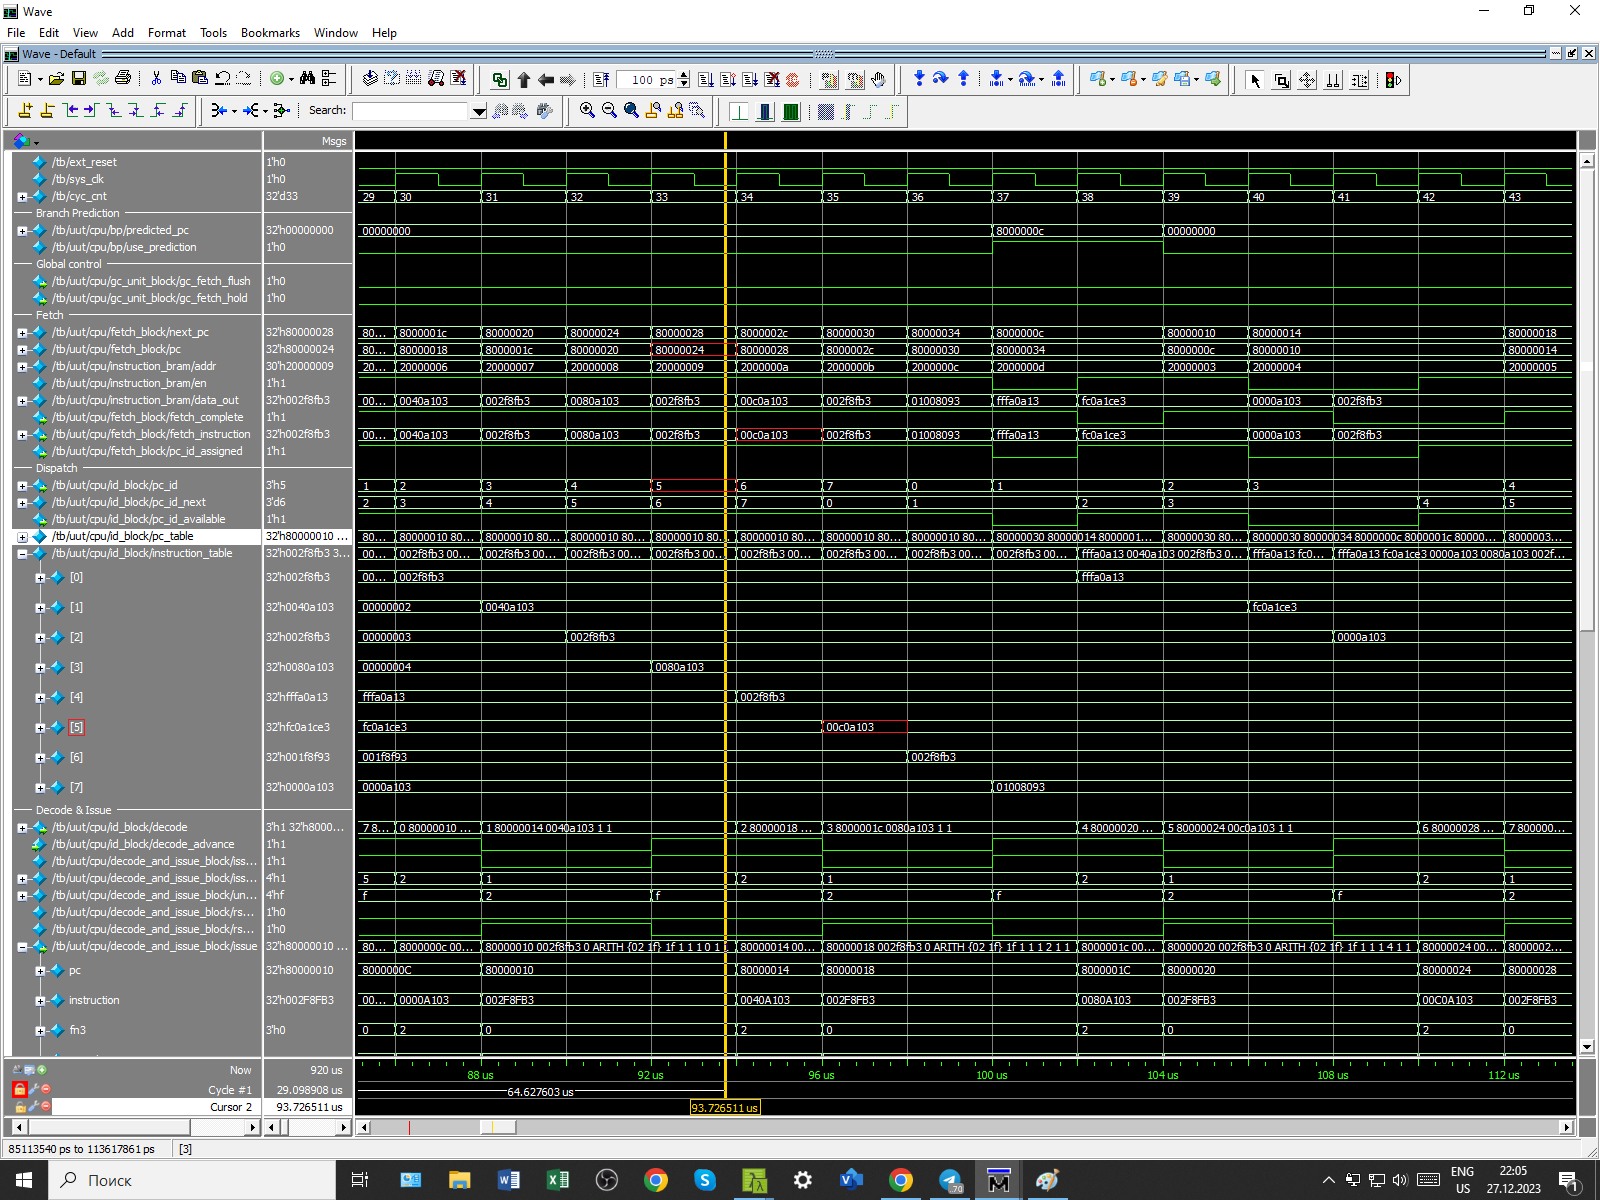
\includegraphics[width=1\textwidth]{img/2.png}
	\caption{Временная диаграмма выполнения стадий выборки и диспечеризации команды по адресу 80000024, 2-я итерация}
	\label{fig:2}
\end{figure}

\subsection{Задание 3}

\begin{figure}[H]
	\centering
	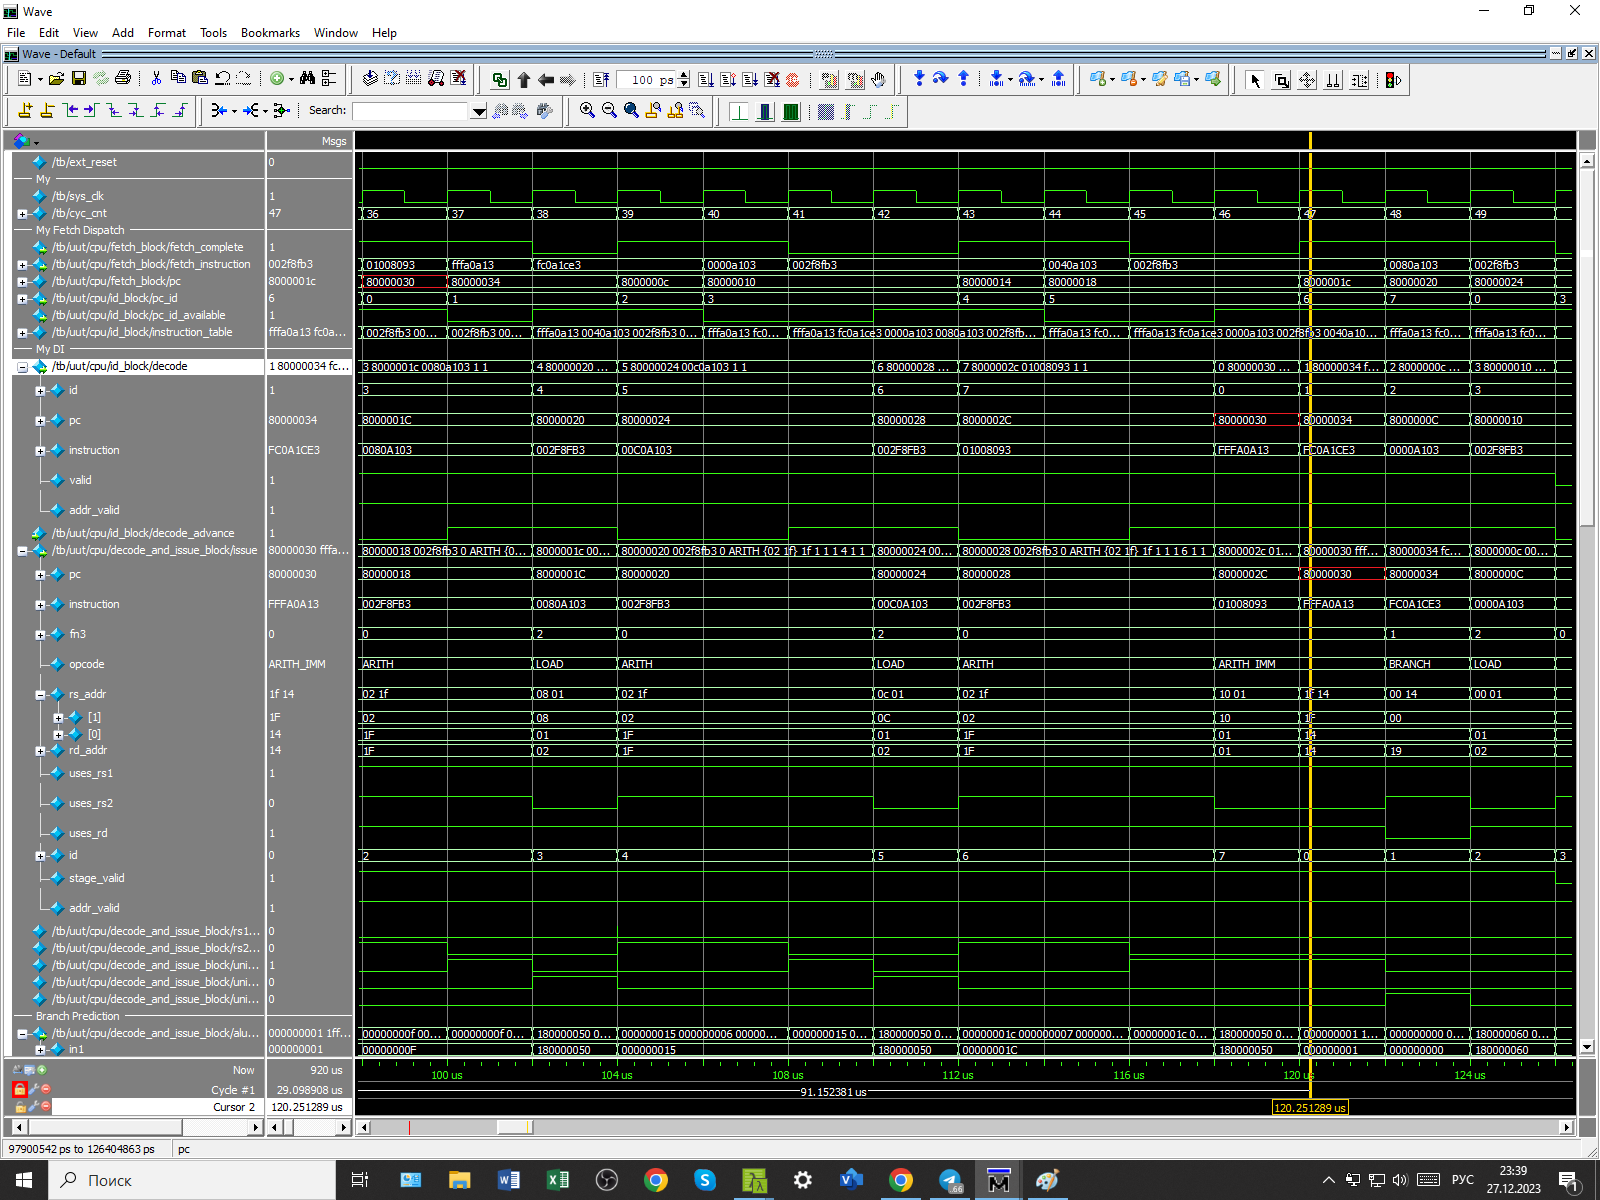
\includegraphics[width=1\textwidth]{img/3.png}
    \caption{Временная диаграмма выполнения стадии декодирования и планирования на выполнение команды по адресу 80000030, 2-я итерация}
	\label{fig:3}
\end{figure}

\subsection{Задание 4}

\begin{figure}[H]
	\centering
	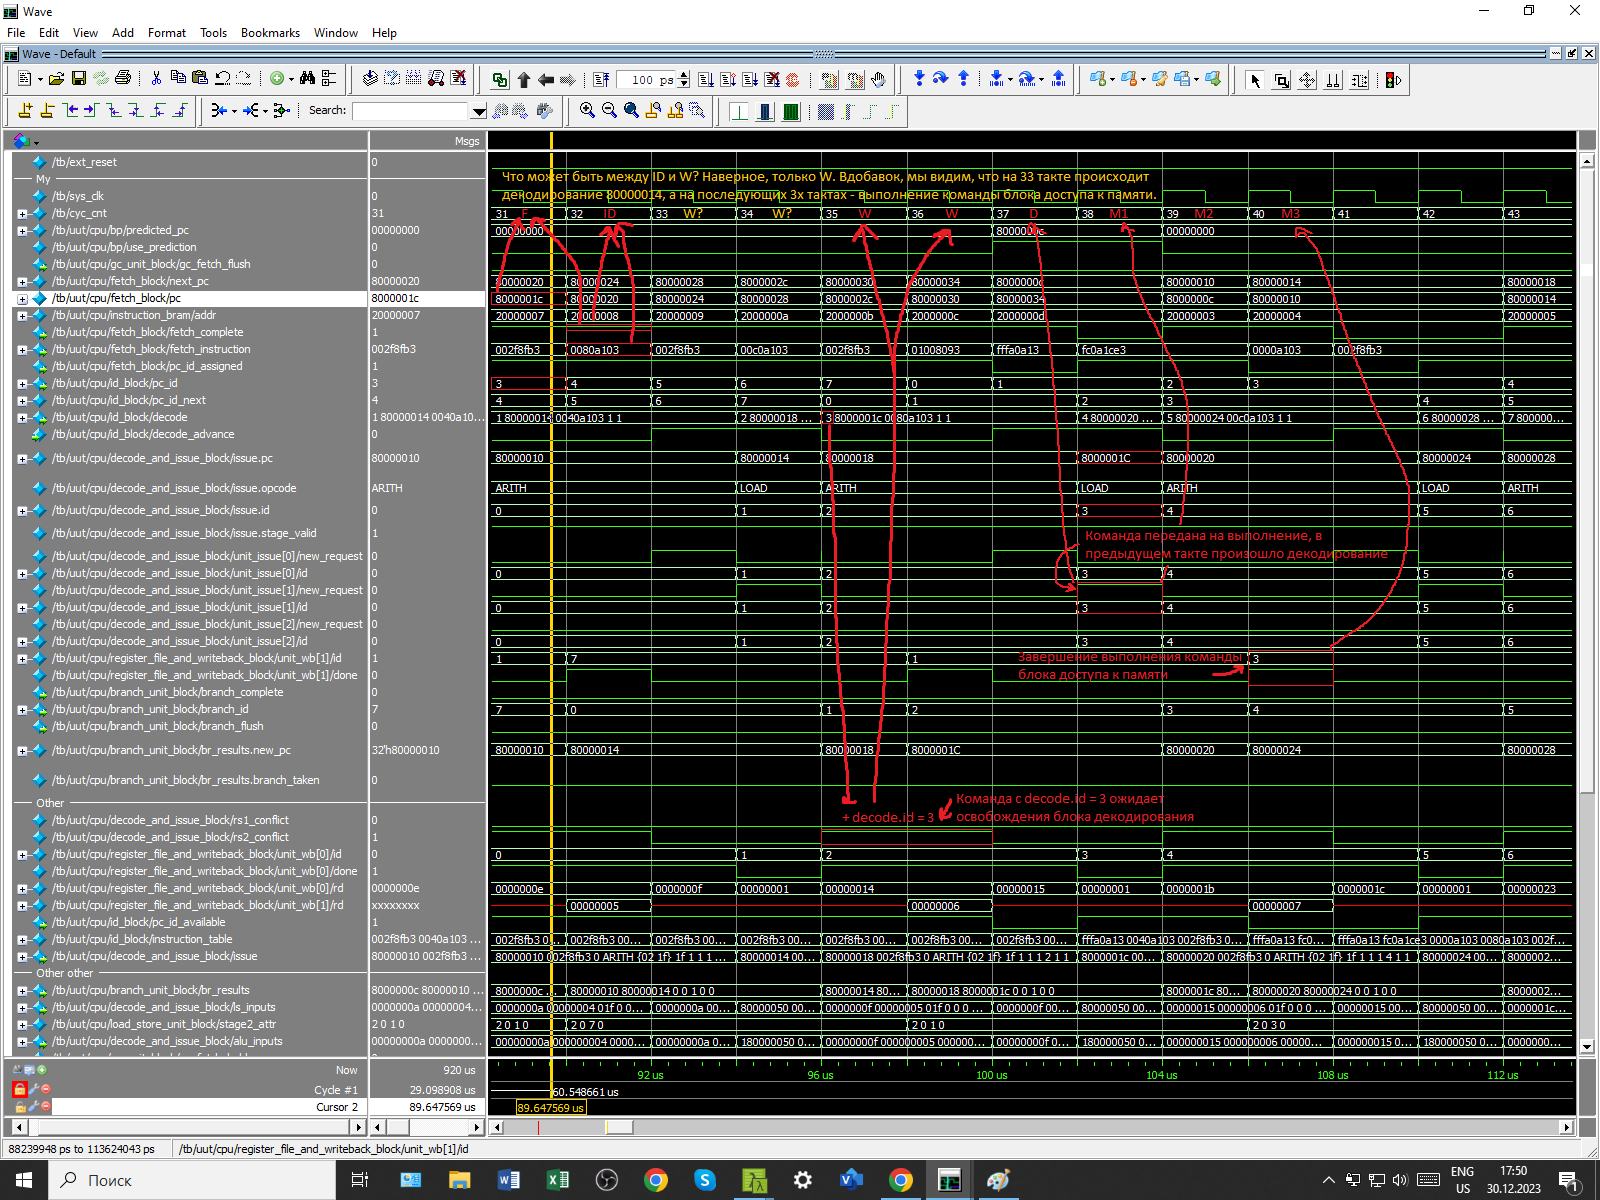
\includegraphics[width=1\textwidth]{img/4.png}
    \caption{Временная диаграмма выполнения стадии выполнения команды по адресу 8000001c, 2-я итерация}
	\label{fig:4}
\end{figure}

\subsection{Задание 5}

\begin{figure}[H]
	\centering
	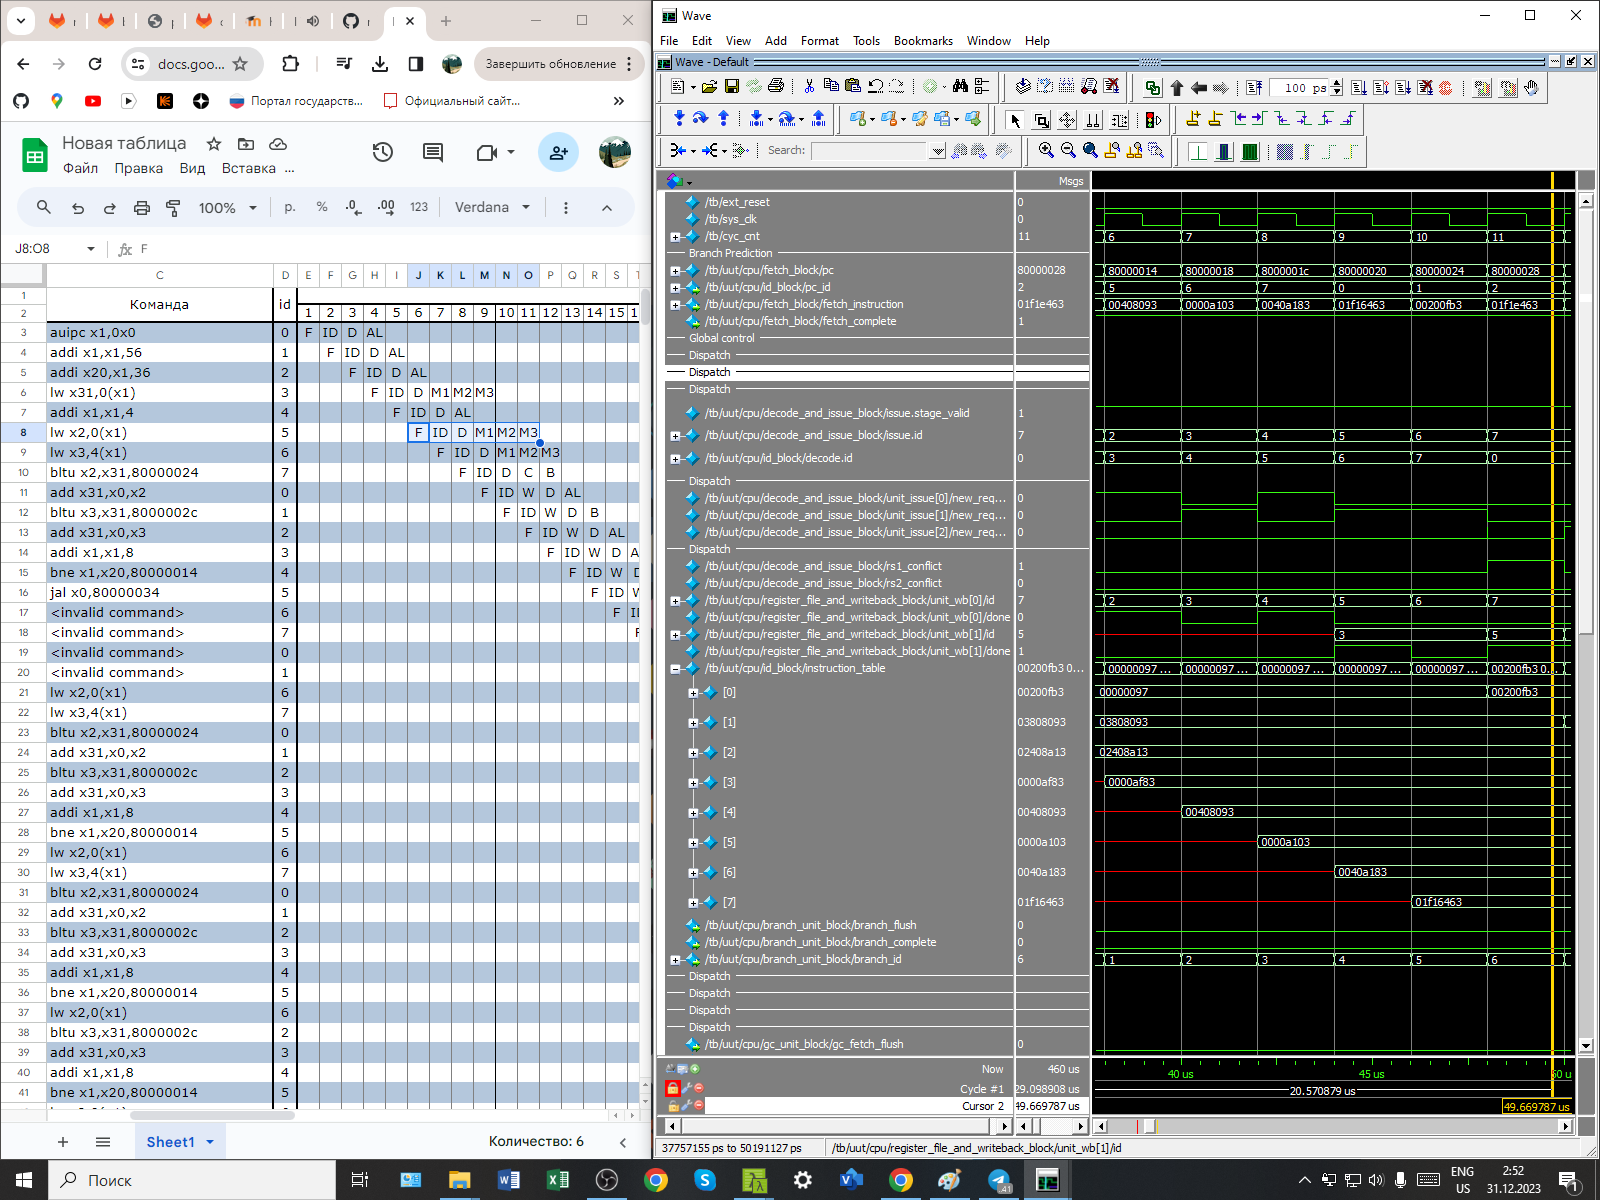
\includegraphics[width=1\textwidth]{img/5.png}
    \caption{Временная диаграмма всех стадий выполнения команды, обозначенной в тексте программы \#!}
	\label{fig:5}
\end{figure}

\begin{figure}[H]
	\centering
	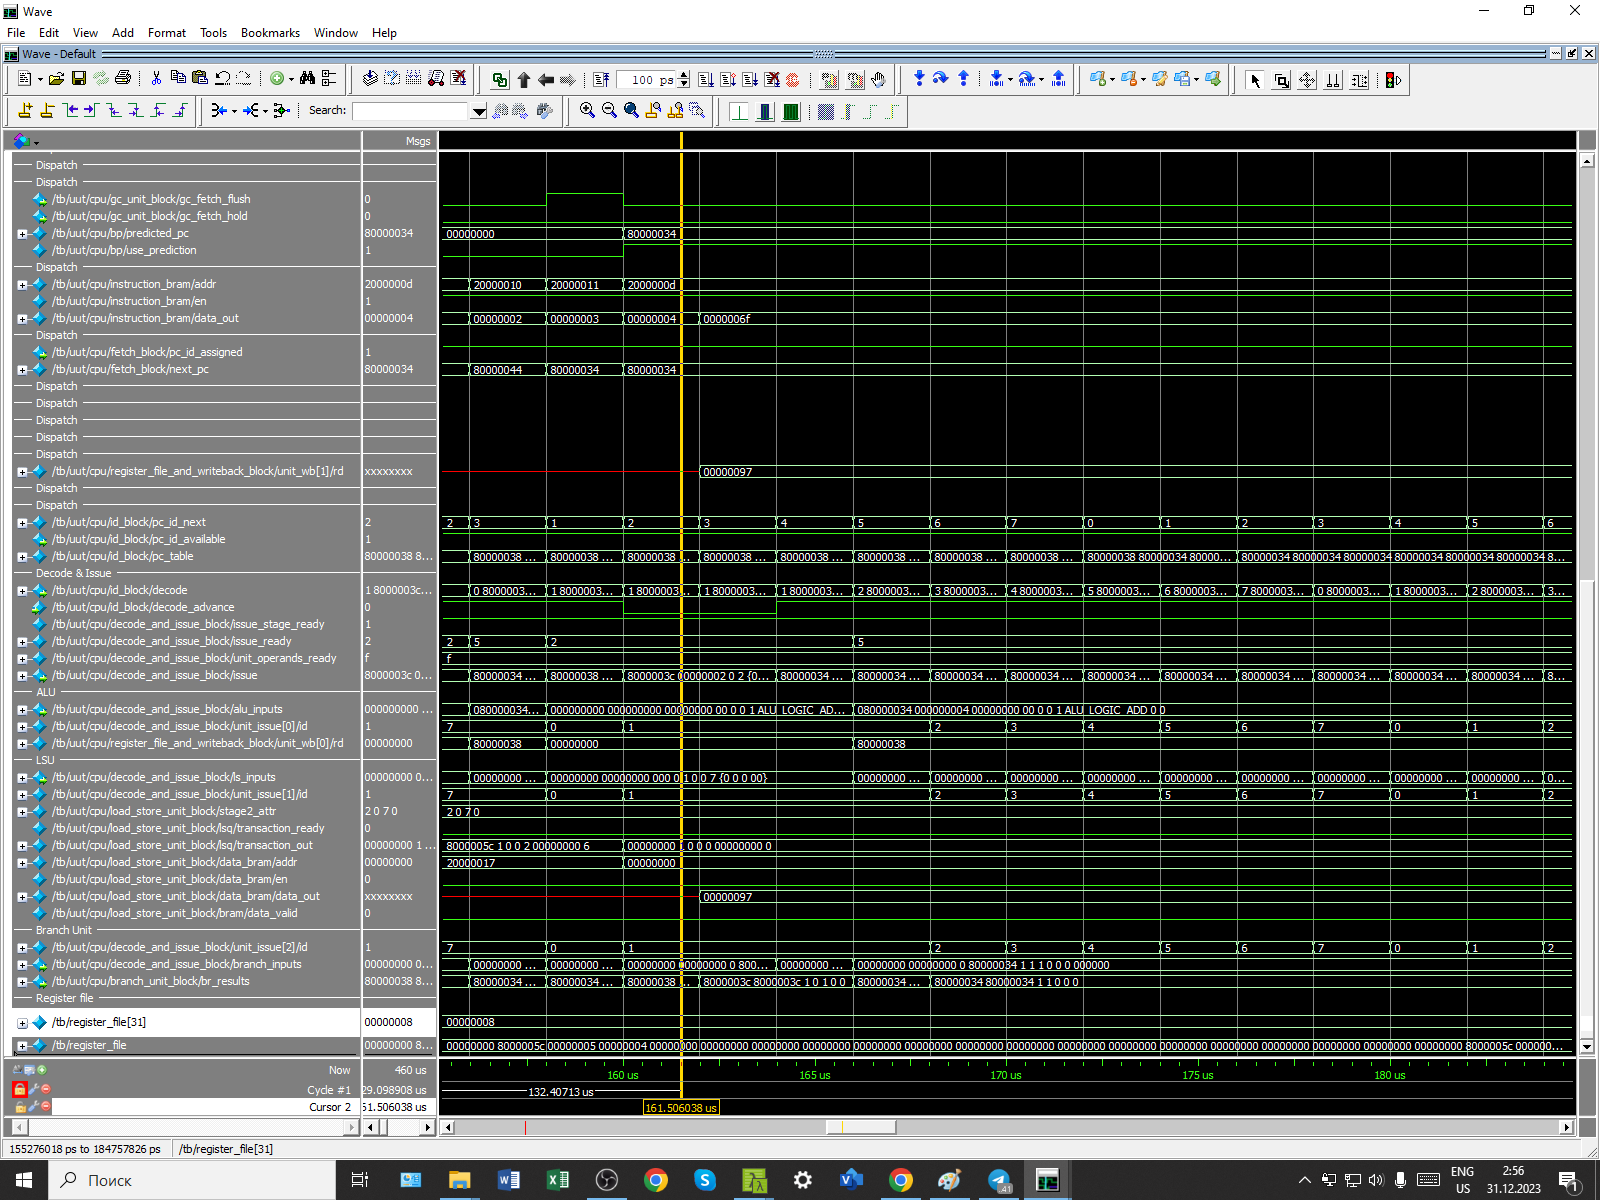
\includegraphics[width=1\textwidth]{img/x31.png}
    \caption{В результате выполнения программы, регистр x31 принимает значение 8, как и ожидалось}
	\label{fig:x31}
\end{figure}

\begin{figure}[H]
	\centering
	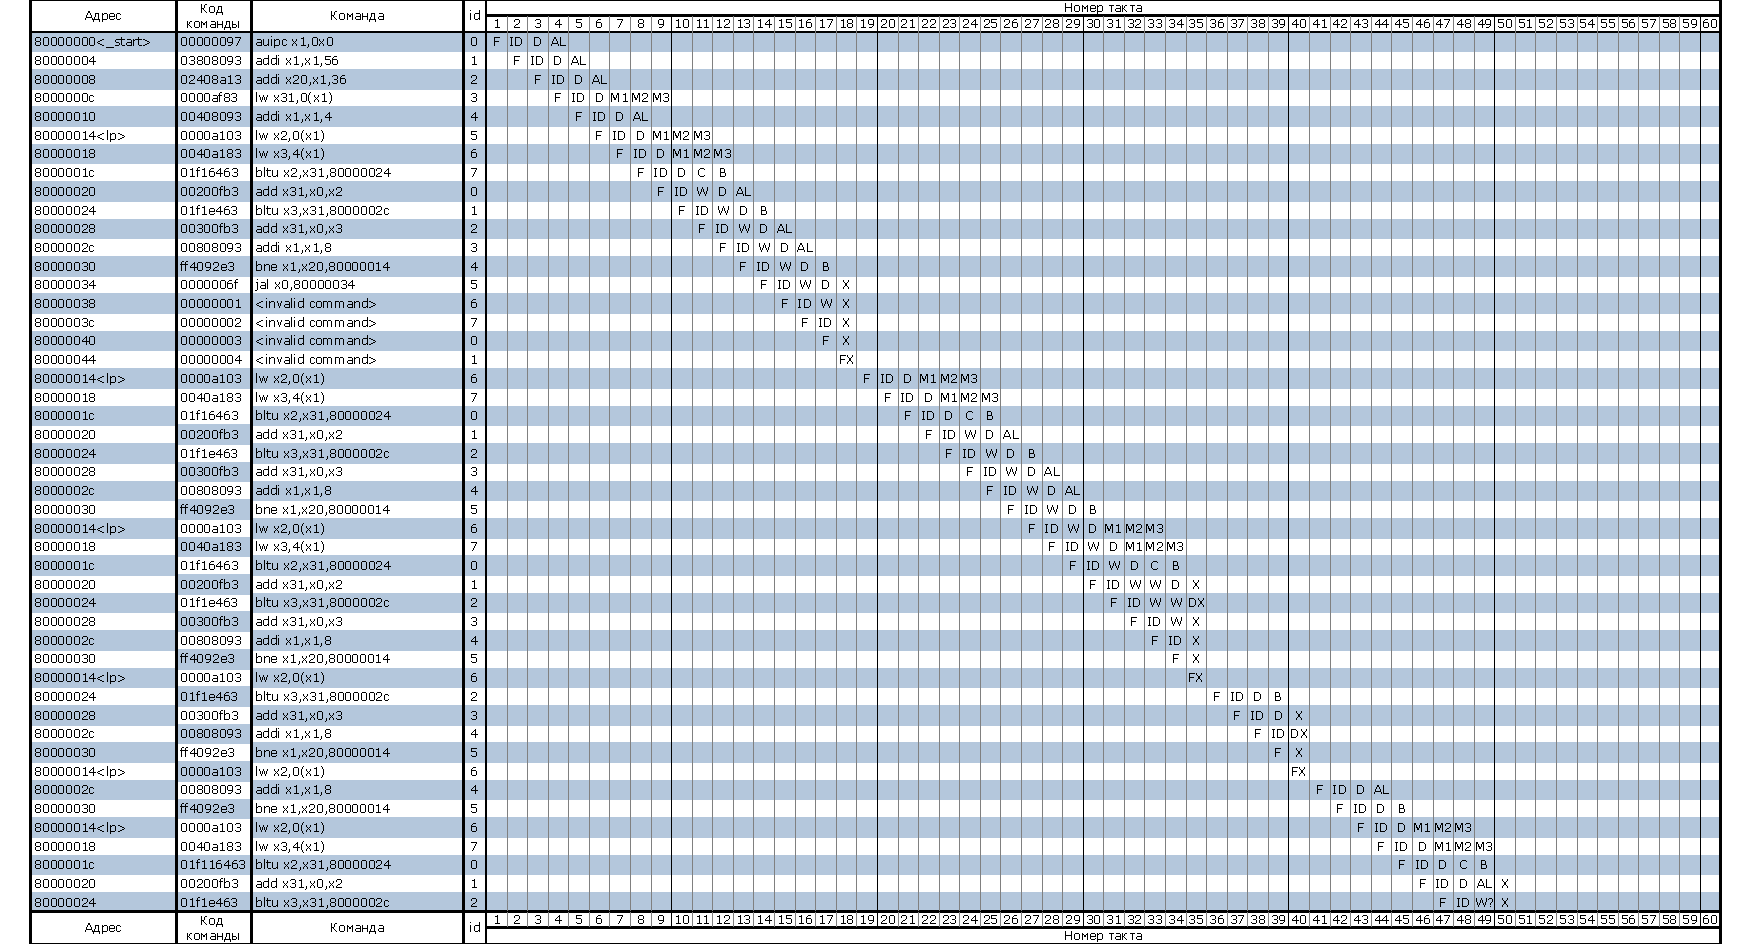
\includegraphics[width=1\textwidth]{img/pipeline-unoptimized.pdf}
    \caption{Трасса выполнения неоптимизированной программы}
	\label{fig:pu}
\end{figure}

Конфликты возникают из-за того, что происходит обращение к регистру, запись в который ещё не была завершена.
Как можно заметить по псевдокоду, строка x1 += enroll (add x1, x1, elem\_sz*enroll) будет выполнена вне зависимости от предшествующих условных переходов, а также значение регистра x1 не используется после строки lw x3, 4(x1) в пределах выполнения тела цикла.
Следовательно, если поместить строку add x1, x1, slem\_sz*enroll сразу после lw x3, 4(x1), это не повлияет на результат выполнения программы, зато даст дополнительную задержку в один такт между загрузкой значения в x2 и чтением из него, что позволит устранить конфликты.

\begin{code}
\begin{lstinputlisting}[
        label={lst:1},
        caption={Оптимизированный код программы по варианту на языке ассемблера}
    ]{lst/opt.s}
\end{lstinputlisting}
\end{code}

\begin{code}
\begin{lstinputlisting}[
        label={lst:1},
        caption={Дизассемблированный листинг оптимизированного кода программы по варианту}
    ]{lst/opt-text.s}
\end{lstinputlisting}
\end{code}

\begin{code}
\begin{lstinputlisting}[
        label={lst:1},
        caption={Оптимизированный код программы по варианту в шестнадцатеричном представлении}
    ]{lst/opt.hex}
\end{lstinputlisting}
\end{code}

\begin{code}
\begin{lstinputlisting}[
        label={lst:1},
        language={C++},
        caption={Псевдокод оптимизированной программы по варианту}
    ]{lst/opt.c}
\end{lstinputlisting}
\end{code}

\begin{figure}[H]
	\centering
	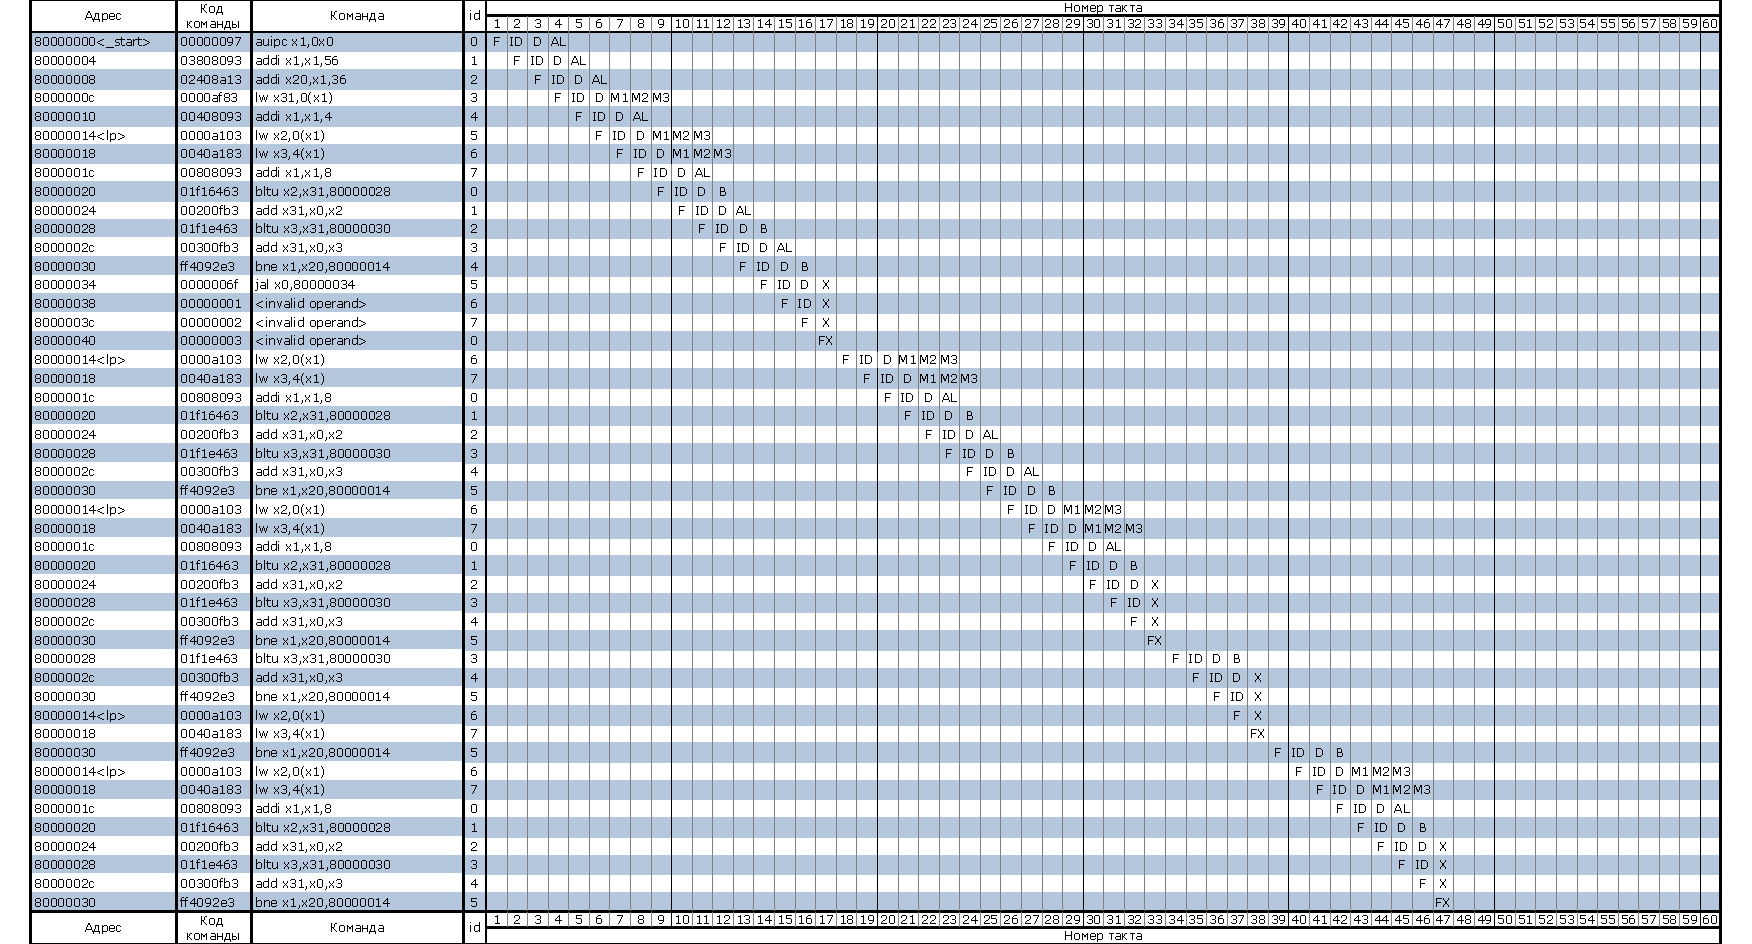
\includegraphics[width=1\textwidth]{img/pipeline-optimized.pdf}
    \caption{Трасса выполнения оптимизированной программы}
	\label{fig:po}
\end{figure}

\newpage

\section{Заключение}

В результате данной работы были изучены принципы функционирования, построения и особенности архитектуры суперскалярных конвейерных микропроцессоров.

На основе изученных материалов был найден способ оптимизировать программу.

Цель работы была достигнута.

\end{document}
